\documentclass{article}

\usepackage[utf8]{inputenc}
\usepackage{geometry}
\usepackage{graphicx}
\usepackage{titling}
\usepackage{fancyhdr}
\usepackage{cmbright}

\geometry{
	a4paper,
	total={170mm, 257mm},
	left=20mm,
	top=20mm
}


\title{Chapter 3: Vehicle 3 - Love}
\author{Fharook Shaik}
\date{19 November 2024}

\fancypagestyle{fancy}{
	\fancyhf{}
	\fancyfoot[R]{
\includegraphics[width=3cm]{images/BTULogo_englisch_grau_2x.png}}
	\fancyfoot[L]{\thedate}
	\fancyhead[L]{13869 - Braitenberg Vehicle Praktium}
	\fancyhead[R]{\theauthor}
}

\pagestyle{fancy}

\makeatletter
\renewcommand{\maketitle}{
	\thispagestyle{fancy}
	\null
	\vskip 1em
	\begin{center}
		{\LARGE \@title \par}
	\end{center}
	\vskip 3em
}
\makeatother


\begin{document}

	\maketitle

	\noindent\begin{tabular}{@{}ll}
		Student & \theauthor\\
		Professor &  Dr. Cunningham, Douglas\\
		Matrikel-Nr.: & 5014962
		 
	\end{tabular}

	\section*{Summary}
	In Chapter 3, Valentino Braitenberg introduces Vehicle 3, a new design that displays behavior resembling love. While Vehicle 2 showed extreme reactions like fear (Vehicle 2a) or aggression (Vehicle 2b), Vehicle 3 is calmer and more balanced. This change is achieved by introducing inhibitory connections between its sensors and motors. Unlike earlier vehicles, the motors slow down when a sensor detects something strong, creating more thoughtful and relaxed behaviors.

    Vehicle 3 comes in two main forms. In Vehicle 3a, the sensors are connected directly to the motors on the same side. When this vehicle senses a strong stimulus, like heat or light, the motor on the side closer to the source slows down. This makes the vehicle turn toward the source and eventually stop directly in front of it. It stays there peacefully, as if admiring the source and wanting to remain near it. This gives Vehicle 3a a personality that feels steady and loyal it \textbf{"loves"} the source in a permanent way.

    Vehicle 3b works differently. Its sensors are connected to the motors on the opposite side (crossed connections). Like Vehicle 3a, it slows down when it detects a strong stimulus, but it stops facing away from the source. This behavior makes it seem less settled it lingers near the source for a while but is easily disturbed and may drift away. It's as though Vehicle 3b is curious, always exploring and keeping an eye out for other sources. This gives it a more dynamic personality, showing a love for the source but also a readiness to find something new.

    \begin{figure}[h]
		\centering
		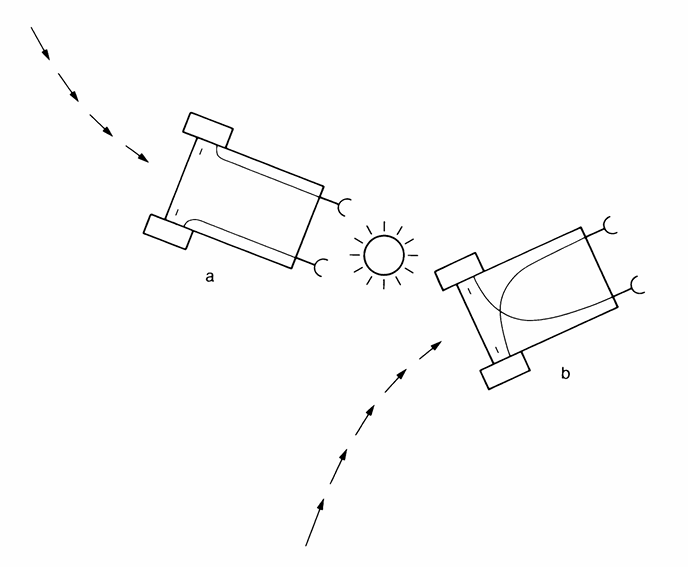
\includegraphics[scale=0.5]{images/Vehicle_3a_3b.png}
		\caption{Vehicle 3 (a) Same-Side connection (b) Crossed connection }
		\label{fig:vehicle-3ab}
	\end{figure}

    Braitenberg then introduces Vehicle 3c, a more advanced version with four pairs of sensors. These sensors can detect various environmental factors such as light, temperature, oxygen, and organic matter. Vehicle 3c combines different types of connections some like Vehicle 2a and 2b, and others like Vehicle 3a and 3b. This creates highly complex behaviors. For example, Vehicle 3c avoids high temperatures by turning away from hot areas, destroys light bulbs (as if it knows they generate heat), and seeks out oxygen rich and nutrient rich locations. It spends most of its time in these favorable areas but moves on when resources run low. Its behavior looks smart, as if it understands its needs and knows how to meet them.

    \newpage

    \begin{figure}[h]
		\centering
		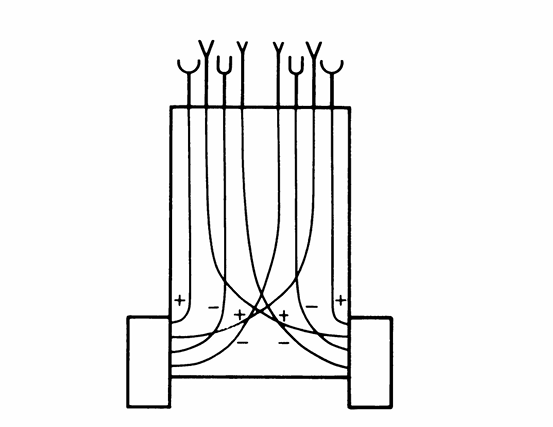
\includegraphics[scale=0.5]{images/Vehicle_3c.png}
		\caption{Vehicle 3 (c) Multisensory Vehicle }
		\label{fig:vehicle-3c}
	\end{figure}

    At first glance, it might seem like Vehicle 3c has values or even knowledge. For instance, it appears to know that light bulbs increase heat or that oxygen and organic matter are important for survival. However, Braitenberg emphasizes that this is an illusion. The behaviors come from the way the sensors and motors interact they're not based on real knowledge or thought. There's no actual understanding or decision-making involved, just simple mechanics creating patterns that seem intentional.

    Braitenberg concludes by discussing the incredible variety of behaviors you can create by tweaking the design of Vehicle 3. Changing the types of sensors, how they connect to the motors, or the strength of their effects opens up endless possibilities. For instance, a vehicle might care more about oxygen than light, or its sense of smell might be stronger for organic matter than for other chemicals. Vehicle 3 shows how even simple designs can produce surprisingly lifelike and complex behaviors, setting the stage for even more sophisticated models in the chapters to come.

\end{document}